% Format teze zasnovan je na paketu memoir
% http://tug.ctan.org/macros/latex/contrib/memoir/memman.pdf ili
% http://texdoc.net/texmf-dist/doc/latex/memoir/memman.pdf
% 
% Prilikom zadavanja klase memoir, navedenim opcijama se podešava 
% veličina slova (12pt) i jednostrano štampanje (oneside).
% Ove parametre možete menjati samo ako pravite nezvanične verzije
% mastera za privatnu upotrebu (na primer, u b5 varijanti ima smisla 
% smanjiti 
\documentclass[12pt,oneside]{memoir} 

% Paket koji definiše sve specifičnosti master rada Matematičkog fakulteta
\usepackage[latinica]{matfmaster} 

\usepackage{listings}
%
% Podrazumevano pismo je ćirilica.
%   Ako koristite pdflatex, a ne xetex, sav latinički tekst na srpskom jeziku
%   treba biti okružen sa \lat{...} ili \begin{latinica}...\end{latinica}.
%
% Opicija [latinica]:
%   ako želite da pišete latiniciom, dodajte opciju "latinica" tj.
%   prethodni paket uključite pomoću: \usepackage[latinica]{matfmaster}.
%   Ako koristite pdflatex, a ne xetex, sav ćirilički tekst treba biti
%   okružen sa \cir{...} ili \begin{cirilica}...\end{cirilica}.
%
% Opcija [biblatex]:
%   ako želite da koristite reference na više jezika i umesto paketa
%   bibtex da koristite BibLaTeX/Biber, dodajte opciju "biblatex" tj.
%   prethodni paket uključite pomoću: \usepackage[biblatex]{matfmaster}
%
% Opcija [b5paper]:
%   ako želite da napravite verziju teze u manjem (b5) formatu, navedite
%   opciju "b5paper", tj. prethodni paket uključite pomoću: 
%   \usepackage[b5paper]{matfmaster}. Tada ima smisla razmisliti o promeni
%   veličine slova (izmenom opcije 12pt na 11pt u \documentclass{memoir}).
%
% Naravno, opcije je moguće kombinovati.
% Npr. \usepackage[b5paper,biblatex]{matfmaster}

% Pomoćni paket koji generiše nasumičan tekst u kojem se javljaju sva slova
% azbuke (nema potrebe koristiti ovo u pravim disertacijama)
% \usepackage[latinica]{pangrami}

% Datoteka sa literaturom u BibTex tj. BibLaTeX/Biber formatu
\bib{matfmaster-primer}

% Ime kandidata na srpskom jeziku (u odabranom pismu)
\autor{Ognjen Ž. Plavšić}
% Naslov teze na srpskom jeziku (u odabranom pismu)
\naslov{RADNI NASLOV}
% Godina u kojoj je teza predana komisiji
\godina{2022}
% Ime i afilijacija mentora (u odabranom pismu)
\mentor{dr Milena \textsc{Vujošević Janičić}, vanredni profesor\\ Univerzitet u Beogradu, Matematički fakultet}
% Ime i afilijacija prvog člana komisije (u odabranom pismu)
\komisijaA{dr Filip \textsc{Marić}, vanredni profesor\\ Univerzitet u Beogradu, Matematički fakultet}
% Ime i afilijacija drugog člana komisije (u odabranom pismu)
\komisijaB{dr Jelena \textsc{Graovac}, docent\\ Univerzitet u Beogradu, Matematički fakultet}
% Ime i afilijacija trećeg člana komisije (opciono)
% \komisijaC{}
% Ime i afilijacija četvrtog člana komisije (opciono)
% \komisijaD{}
% Datum odbrane (odkomentarisati narednu liniju i upisati datum odbrane ako je poznat)
% \datumodbrane{}

% Apstrakt na srpskom jeziku (u odabranom pismu)
\apstr{%
% \pangrami
}

% Ključne reči na srpskom jeziku (u odabranom pismu)
\kljucnereci{računarstvo, autosar, clang, llvm, c++}

\begin{document}
% ==============================================================================
% Uvodni deo teze
\frontmatter
% ==============================================================================
% Naslovna strana
\naslovna
% Strana sa podacima o mentoru i članovima komisije
\komisija
% Strana sa posvetom (u odabranom pismu)
\posveta{Porodici}
% Strana sa podacima o disertaciji na srpskom jeziku
\apstrakt
% Sadržaj teze
\tableofcontents*

% ==============================================================================
% Glavni deo teze
\mainmatter
% ==============================================================================

% ------------------------------------------------------------------------------
\chapter{Uvod}
% ------------------------------------------------------------------------------
% \pangrami

% \section{Primeri korišćenja klasičnih \LaTeX{} elemenata}
% % Primeri citiranja
% Još jedan citat \cite{GuSh:243}.
% % Primeri navodnika
% Isprobavamo navodnike: "Rekao je da mu se javimo sutra".
% % Primer referisanja na tabelu (koja se javlja kasnije)
% U tabeli \ref{tbl:rezultati} koja sledi prikazani su rezultati eksperimenta.
% % Primer kraćeg ćiriličkog teksta
% {\cir Ово је пример ћириличког текста који се јавља у латиничком документу.}
% U ovoj rečenici se javlja jedna reč na {\cir ћирилици}.
% % Primer korišćenja fusnota
% Iza ove rečenice sledi fusnota.\footnote{Ovo je fusnota.}

% % Primer dužeg ćirličkog teksta
% \begin{cirilica}
%   Ово је мало дужи блок текста исписан ћириличким писмом у оквиру
%   латиничког документа. Фијуче ветар у шибљу, леди пасаже и куће иза
%   њих и гунђа у оџацима.
% \end{cirilica}

% % Primer korišćenja tabele
% \begin{table}
% \centering
% \caption{Rezultati}
% \label{tbl:rezultati}
% \begin{tabular}{c>{\centering}p{2cm}c}
% \toprule
% 1 & 2 & 3\\\midrule
% 4 & 5 & 6\\\cmidrule(rl){1-2}
% 7 & 8 & 8\\
% \bottomrule
% \end{tabular}
% \end{table}

% % Primer korišćenja slike
% \begin{figure}[!ht]
%   \centering
%   \label{fig:grafikon}
%   \includegraphics[width=0.5\textwidth]{graph.png}
%   \caption{Grafikon}
% \end{figure}


% % Primer jednostavnije matematičke formule
% Evo i jedan primer matematičke formule: $e^{i\pi} + 1 = 0$. 
% % Primer referisanja na sliku
% Na slici \ref{fig:grafikon} prikazan je jedan grafikon.

% % primer kompleksnije matematičke formule
% $$
% \int_a^b f(x)\ \mathrm{d}x \ =_{def}\ \lim_{\max{\Delta x_k \rightarrow 0}} \sum_{k=1}^n f(x_k^*)\Delta x_k
% $$

% % primer referisanja na poglavlja i strane poglavlja
% Više detalja biće dato u glavi \ref{chp:razrada} na strani \pageref{chp:razrada}.

% % primer liste
% Možemo praviti i nabrajanja:
% \begin{enumerate}
% \item Analiza 1
% \item Linearna algebra
% \item Analitička geometrija
% \item Osnovi programiranja
% \end{enumerate}

% \pangrami

% ------------------------------------------------------------------------------
\chapter{Autosar C++14 standard kodiranja}
\label{chp:autosar}

AUTomotive Open System ARchitecture (AUTOSAR) je razvojno partnerstvo proizvodjača vozila, dobavljača, pružaoca usluga i kompanija iz automobilske industrije i industrija elektronike, poluprovodnika i softvera na globalnom nivou \cite{AutosarWebsite}. 
Cilj Autosara je da stvori i uspostavi otvorenu i standardizovanu softversku arhitekturu za automobilske elektronske upravljačke jedinice (ЕCU).
Radi ostvarenja pomenutih ciljeva AUTOSAR definiše, izmedju ostalog, pravila kodiranja u programskom jeziku C++14 za sigurnosna i kritična okruženja. Glavni sektor primene AUTOSAR C++14 standarda kodiranja je automobilska industrija, medjutim ovaj standard može biti primenjen
i na druge ugradjene (\textit{eng. embedded}) aplikacije. Pomenuti standard predstavlja nadogradnju postojećeg MISRA C++:2008 standarda \cite{AutosarGuidelines}.

\section{Klasifikacija pravila}
AUTOSAR C++14 standard definiše 342 pravila od kojih je 154 prisvojeno bez modifikacija od MISRA C++:2008 standarda, 131 su prisvojeni
iz drugih C++ standarda i 57 pravila je zasnovano na istraživanju, literaturi ili iz drugih resursa.

Pravila su klasifikovana po nivou obaveze, mogućnosti ispitivanja saglasnosti koda sa pravilom korišćenjem algoritama
statičke analize i cilju korišćenja.
\indent
Klasifikacija po nivou obaveze deli pravila na obavezna i preporučena.
Obavezna pravila predstavljaju neophodne zahteve koje C++ kod mora ispuniti kako bi bio u saglasnosti sa standardom. U slučaju kada ovo nije moguće,
formalna odstupanja moraju biti prijavljena.
Preporučena pravila predstavljaju zahteve koje C++ kod treba ispuniti kad god je to moguce. Medjutim, ovi zahtevi nisu obavezni. Pravila
sa ovim nivoom obaveze ne treba smatrati savetom ili sugestijom koja može biti ignorisana i treba ih pratiti kad god je to 
izvodljivo u praksi. Za ova pravila ne moraju biti prijavljena formalna odstupanja.

Klasifikacija po primenjivosti statičke analize deli pravila na automatizovana, delimično automatizovana i neautomatizovana.
Automatizovana su ona pravila kod kojih se ispitivanje saglasnosti koda može u potpunosti automatizovati algoritmima statičke analize.
Kod delimično automatizovanih pravila se ispitivanje saglasnosti koda može samo delimilčno automatizovati, na primer, korišćenjem neke heuristike ili pokrivanjem određenog broja slučajeva upotrebe i služi kao dopuna manuelnog pregleda koda.
Za neautomatizovana pravila statička analiza ne pruža razumnu podršku. Za ispitivanje saglasnosti koda sa neautomatizovanim pravilima koriste se druga sredstva, kao što su manuelni pregled koda ili drugi alati.

\indent
Većina pravila iz Autosar C++14 standarda spadaju u Automatizovana pravila. Alati za statičku analizu koda koji tvrde da podržavaju Autosar C++14 standard moraju u potpunosti obezbediti podršku za sva Automatizovana pravila i delimičnu podršku, u meri u kojoj je to moguće, za pravila koja se ne mogu u potpunosti ispitati algoritmima statičke analize \cite{AutosarGuidelines}.

\indent
Primenjivost statičke analize na proveru saglasnosti koda sa odredjenim pravilom u velikoj meri zasniva se na teorijskoj klasifikaciji problema
na odlučive i neodlučive. Ukoliko se pravilo zasniva na neodlučivom problemu, odnosno dokazano je da ne postoji algoritam koji bi u konačnom broju koraka odgovorio sa DA ili NE na pomenuti problem, možemo sa sigurnošću reći da alati za statičku analizu nisu u mogućnosti da u
potpunosti ispitaju saglasnost koda sa ovim pravilom. Pravilo će verovatno biti klasifikovano kao parcijalno automatizovano ili neautomatizovano ukoliko detektovanje kršenja pravila obuhvata odredjivanje vrednosti koju promenljiva sadrži ili da li program doseže odredjeni deo programa.

Primer parcijalno automatizovanog pravila je: 
\begin{verbatim}
Pravilo M5-8-1 (obvezno, implementaciono, parcijalno automatizovano) 
Desni operand šift operacije treba biti manji izmedju nula i jedan
od bitske širine tipa levog operanda.
\end{verbatim}
  % \textit{Pravilo M5-8-1 (obvezno, implementaciono, parcijalno automatizovano)
  %         Desni operand šift operacije treba biti manji izmedju nula i jedan od bitske širine tipa levog operanda.} \\ \\
  Pravilo nije moguće u potpunosti automatizovati jer je očigledno potrebno poznavati vrednost desnog operanda, što u opštem slučaju nije
  moguće zaključiti. Primer ovakvog koda prikazan je na listingu 2.1. 
\begin{english}
\lstset{%
language=C,
frame=single,
numbers=left,
numberstyle=\footnotesize,
tabsize=2,
keepspaces=true,
columns=fullflexible,
basicstyle=\ttfamily\scriptsize,
keywordstyle=\color{blue}
}



\begin{lstlisting}[caption={Kod koji ilustruje nemogućnost primene statičke analize},label={lst:label},language=C++, captionpos=b]
#include <iostream>
#include <cstdint>
#include <cstdlib>

int main(){
int8_t u8a = rand() % 100;
u8a = (uint8_t) ( u8a << rand() % 10);
}
\end{lstlisting}
\end{english}
Medjitim, ukoliko je desni operand konstanta ili constexpr promenljiva, vrlo je verovatno da će alat za statičku analizu biti u stanju
  da zaključi vrednost ove promenljive (s obzirom da su ove vrednosti poznate tokom kompilacije), a samim tim i ispitati saglasnost koda sa ovim pravilom.
  Primer ovakvog koda prikazan je na Listingu 2.2.
\begin{english}
\lstset{%
language=C,
frame=single,
numbers=left,
numberstyle=\footnotesize,
tabsize=2,
keepspaces=true,
columns=fullflexible,
basicstyle=\ttfamily\scriptsize,
keywordstyle=\color{blue}
}



\begin{lstlisting}[caption={Kod čija se ispravnost jednostavno može utvrditi statičkom analizom},label={lst:label},language=C++, captionpos=b]
#include <iostream>
#include <cstdint>
#include <cstdlib>

int main(){
int8_t u8a = rand() % 100;
u8a = (uint8_t) ( u8a << 7);
}
\end{lstlisting}
\end{english}

  Napredniji alati za statičku analizu koji podržavaju simboličko izvršavanje programa (npr. Clang Static Analyzer) mogu pokriti i znatno kompleksnije 
  slučajeve od slučaja prikazanog u Listingu 2.2.
  \\
  \indent 
  Ukoliko su pravila koja se odnose na implementaciju C++ projekta, odnosno na C++ konstrukte i semantiku programa, dovoljno kompleksna, može se desiti da u potpunosti nije moguće koristiti alate za statičku analizu. Ovo uglavnom znači da je broj slučajeva upotrebe koji algoritmi iz statičkih alata mogu pokriti, zanemarljiv. Medjutim, odredjeni broj pravila koja su klasifikovana kao Neautomatizovana odnose se na aspekte koda koji zavise od samog projekta
  u okviru kog je kod napisan, stoga je nemoguće koristiti algoritme statičke analize.
  Primer ovakvog pravila je:
  \begin{verbatim}
Pravilo A1-4-2 (obvezno, implementaciono, neautomatizovano)
Sav kod treba poštovati definisane granice metrika koda.
\end{verbatim}

  %  \\ \\
  % \textit{Pravilo A1-4-2 (obvezno, implementaciono, neautomatizovano)
  %         Sav kod treba poštovati definisane granice metrika koda.} \\

  Kako bi se odredilo da li je kod napisan u skladu sa ovim pravilom, očigledno je potrebno poznavati koje metrike koda se koriste u okviru projekta i
  granice definisane za te metrike. S obzirom da je ovo specifično za sam projekat, mogu se koristiti interni alati za statičku analizu koda u kombinaciji
  sa manuelnim pregledom koda. 

Klasifikacija pravila prema cilju primene (slučaju upotrebe) deli pravila na implementaciona, verifikaciona, pravila za alate i infrastrukturna.
Implementaciona su ona pravila koja se odnose na samu implementaciju projekta odnosno na kod, arhitekturu i dizajn.
Verifikaciona pravila odnose se na proces verifikacije koji uključuje pregled koda, analizu i testiranje.
Pravila za alate odnose se na softverske alate kao što su pretprocesor, kompajler, linker i biblioteke kompajlera.
Infrastrukturna su ona pravila koja se odnose na operativni sistem i hardver \cite{AutosarGuidelines}.


\section{Opis implementiranih pravila}

Pored formalne klasifikacije opisane u prethodnom poglavlju, pravila u okviru samog dokumenta AUTOSAR C++14 standarda kodiranja struktuirana su po poglavljima.
Struktura poglavlja ovog dokumenta slična je strukturi iz samog C++ standarda ISO/IEC 14882:2014. Svako poglavlje odgovara jednoj komponenti (svojstvu) C++14 jezika, to jest, sadrži pravila koja se odnose na tu komponentu.
\\
\indent
Pravila razmatrana u ovom radu predstavljaju podskup pravila koja se odnose na deklaracije. Razlog za ovo je dvojak. Deklaracije predstavljaju jedan
od osnovnih i najvažnijih koncepta u C++-u i programiranju generalno. U C++-u deklaracije čine samu srž ekspresivne moći jezika i u direktnoj su vezi
sa naprednijim konceptima jezika i računarastva, kao što je, na primer, šablonsko metaprogramiranje (\textit{eng. template metaprogramming}).
Sa druge strane jednostavnost sintakse deklaracija u C++-u čini pogodno tlo za korišćenje kompajlerskih tehnika i struktura u okviru Clang kompajlera kojim se mogu analizirati konstrukti jezika koji nisu u skladu sa pravilima i predlagati prikladne alternative.
\\
\indent
Sva implementirana pravila u okviru projekta spadaju, prema klasifikaciji iz prethodnog poglavlja, u sledeće kategorije:
\begin{enumerate}
  \item{Obavezna, prema klasifikaciji po obavezi.}
  \item{Automatizovana, prema klasifikaciji po primenjivosti statičke analize.}
  \item{Implementaciona, prema klasifikaciji po cilju primene.}
\end{enumerate}

Razmatrana pravila nisu nužno implementirana u potpunosti u okviru Autofix alata, iako činjenica da pravila spadaju u kategorije obaveznih i automatizovanih
implicira da je to teorijski moguće uraditi. Pravila koje Autofix podržava birana su tako da se ograničenja koja potiču iz same prirode projekta minimalno manifestuju. Ograničenja potiču od primarnih tehnologija i biblioteka kojima je alat implementiran ali i činjenice da se alat zasniva na predlogu izmena koda. 
Clang Statički analizator (\textit{eng. Clang Static Analyzer}) nije korišćen u okviru ovog alata, tako da su pravila izabrana tako da što manji broj slučajeva upotrebe zahteva simboličko izvršavanje programa. Drugo ograničenje potiče iz činjenice da u nekim slučajevima nije moguće ili je znatno komplikovanije kreirati predlog ispravke koda (\textit{eng. fixit hint}). Pravila razmatrana u okviru ovog rada birana su tako da se većina konstrukta koji nisu u saglasnosti sa pravilom mogu detektovati analizom Clang-ovog AST-a i da se za njih mogu kreirati razumne alternative koje su u skladu sa Autosar C++14 standardom.
Primeri pravila koje podržava Autofix alat prikazani su na slikama 2.1 i 2.2.

% primer korišćenja slike
\begin{figure}[!ht]
  \centering
  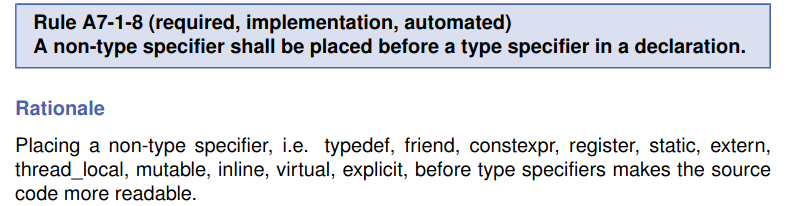
\includegraphics[width=0.5\textwidth]{PraviloA718.png}
  \caption{Pravilo A7-1-8}
  \label{fig:grafikon}
\end{figure}

\begin{figure}[!ht]
  \centering
  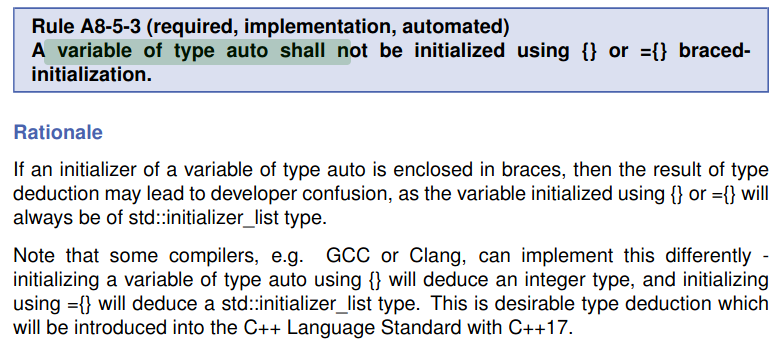
\includegraphics[width=0.5\textwidth]{PraviloA853.png}
  \caption{Pravilo A8-5-3}
  \label{fig:grafikon}
\end{figure}

\chapter{LLVM (nije spremno za reivew)}
\label{chp:llvm}

LLVM projekat predstavlja kolekciju modularnih i ponovo iskoristivih kompajlerskih tehnologija i alata.
Započet je 2000. godine kao instražički projekat Krisa Latnera (\textit{eng. Chris Lattner}) i Vikrama Advea (\textit{eng. Vikram Adve}) na Univerzitetu Ilinois.

LLVM podržava kompilaciju različitih programskih programiskih jezika na mnoštvo različitih arhitektura hardvera. Jednostavnost dodavanja podrške kompilacije programskog jezika za hardversku arhitekturu omogućeno je fleksibilnim dizajnom kod kog je infrastruktura kompajlera ugrubo podeljena na 3 dela. Izvorni kod podržanih jezika prevodi se u LLVM medjukod bibliotekama koji predstavljaju prednji deo kompajlera (\textit{eng. frontend}). Zatim se nad medjukodom vrši niz optimizacija koje su nezavisne od izvornog koda ali i ciljne arhitekture. Biblioteke koje implementiraju pomenute optimizacije čine srednji deo (\textit{eng. middleend}) infrastrukture LLVM-a. Poslednji deo dizajna čini zadnji deo (\textit{eng. backend}) kompajlera prilikom kog se generiše izvršni kod za ciljnu arhitekturu od LLVM medjukoda.

\section{Clang}

Clang projekat predstavlja prednji deo (\textit{eng. frontend}) LLVM kompajlerske infrastrukture za C familiju jezika (C, C++, Objective C/C++, OpenCL ...).
Pored optimizacija i efikasnog generisanja LLVM medjukoda karakterističan je po ekspresivnosti dijagnostike odnosno kvalitetu poruka upozorenja i grešaka prijavljenih za izvorni kod. Dizajn Clang-a se sastoji od mnoštva biblioteka od kojih su najznačajnije za dizajn sledeće:

\begin{enumerate}
  \item{Lekser i Predprocesor \\
       Implementira leksičku analizu i predprocesiranje.
       Pruža mogućnost uključivanja datoteka zaglavlja, proširenja makroa, uslovne kompilacije i kontrole linija. 
       Kreira niz tokena od sintakse izvornog koda.}
  \item{Parser \\
        Kreira Apstraktno Sintaksno Stablo (AST) \textit{eng. Abstract Syntax Three} od tokena koji su dobijeni leksičkom analizom}
        Clang-ov parser implementiran je kao parser rekurzivnog spuštanja, odnosno analizira izvorni kod od vrha prema dnu nizom rekurzivnih funkcija.

  % \item{Implementaciona, prema klasifikaciji po cilju primene.}
\end{enumerate}



% ------------------------------------------------------------------------------

% \pangrami

% \pangrami

% ------------------------------------------------------------------------------
\chapter{Zaključak}
% ------------------------------------------------------------------------------
% \pangrami

% \pangrami

% ------------------------------------------------------------------------------
% Literatura
% ------------------------------------------------------------------------------
\literatura

% ==============================================================================
% Završni deo teze i prilozi
\backmatter
% ==============================================================================

% ------------------------------------------------------------------------------
% Biografija kandidata
\begin{biografija}
  % \textbf{Ognjen Plavšić} (\emph{Tršić,
  %   26. oktobar/6. novembar 1787. — Beč, 7. februar 1864.}) bio je
  % srpski filolog, reformator srpskog jezika, sakupljač narodnih
  % umotvorina i pisac prvog rečnika srpskog jezika.  Vuk je
  % najznačajnija ličnost srpske književnosti prve polovine XIX
  % veka. Stekao je i nekoliko počasnih mastera.  Učestvovao je u
  % Prvom srpskom ustanku kao pisar i činovnik u Negotinskoj krajini, a
  % nakon sloma ustanka preselio se u Beč, 1813. godine. Tu je upoznao
  % Jerneja Kopitara, cenzora slovenskih knjiga, na čiji je podsticaj
  % krenuo u prikupljanje srpskih narodnih pesama, reformu ćirilice i
  % borbu za uvođenje narodnog jezika u srpsku književnost. Vukovim
  % reformama u srpski jezik je uveden fonetski pravopis, a srpski jezik
  % je potisnuo slavenosrpski jezik koji je u to vreme bio jezik
  % obrazovanih ljudi. Tako se kao najvažnije godine Vukove reforme
  % ističu 1818., 1836., 1839., 1847. i 1852.
\end{biografija}
% ------------------------------------------------------------------------------

\end{document}
